\section{ОПИСАНИЕ ПРЕДМЕТНОЙ ОБЛАСТИ, АНАЛИЗ И ВЫБОР МЕТОДОВ РЕШЕНИЯ ЗАДАЧ}
\ESKDsignature{\normalsize Описание предметной области, анализ и выбор методов решения задач}
\eskdrerun{}
\label{sec:software_design}

\subsection{Цель разработки}
\label{subsec:goal}

Целью работы является создание \textbf{нейронечёткой системы с non--singleton-входами}, обеспечивающей полный цикл экспериментирования: от загрузки и предобработки пользовательских данных до настройки правил, оптимизации гиперпараметров и выбора метода дефаззификации.  

\begin{table}[h]
\centering\small
\caption{Функциональные требования к системе}
\label{tab:req}
\begin{tabular}{p{0.25\linewidth}p{0.65\linewidth}}
\toprule
Требование & Краткое описание \\
\midrule
\textbf{Загрузка данных} & Импорт CSV, Parquet, Excel; поддержка больших наборов с ленивой обработкой (Dask, Polars).\\
\textbf{Предобработка} & Ресэмплирование, нормализация, балансировка, удаление выбросов.\\
\textbf{Выбор термов} & Настраиваемое число и тип термов для каждого признака.\\
\textbf{Выбор классов} & Задание числа классов и их семантических меток.\\
\textbf{База правил} & Конфигурирование вида правил и начальных параметров.\\
\textbf{Границы поиска} & Определение диапазонов для оптимизируемых параметров.\\
\textbf{Оптимизация} & \texttt{Optuna}; в перспективе~--- генетический алгоритм, Bayesian Optimization и~др.\\
\textbf{Функции принадлежности} & Поддержка различных семейств~MF для антецедентов и консеквентов.\\
\textbf{Дефаззификация} & Центроид, биссектор, MOM, SOM, LOM, высота и др. \\
\bottomrule
\end{tabular}
\end{table}

\subsection{Введение в нечёткую логику}
Нечёткая логика --- это математико-концептуальный аппарат для формализации, представления и обработки знаний в условиях лингвистической и экспериментальной неопределённости. В классической булевой логике любое высказывание принимается за истинное или ложное, что не всегда адекватно отражает «размытые» категории реального мира. В 1965 году Л.~Заде предложил обобщить классическую теорию множеств, введя функцию принадлежности
\[
  \mu_A: U \to [0,1],
\]
где \(\mu_A(x)\) интерпретируется как степень истинности высказывания «\(x\) принадлежит множеству \(A\)» \cite{Zadeh1965}. Это позволило:
\begin{itemize}
  \item задавать лингвистические термы («низкий», «средний», «высокий») и получать количественные оценки «примерно 0.7»;
  \item моделировать шум и погрешности измерений при помощи плавных функций принадлежности;
  \item формировать правила «если–то» с мягким порогом срабатывания.
\end{itemize}


\subsubsection{Ключевые области применения}
\label{subsec:applications}

\paragraph{Системы управления и автоматизация}
\begin{itemize}
  \item \emph{Климат-контроль} в зданиях и автомобилях: плавное регулирование температуры и вентиляции;
  \item \emph{Промышленные роботы}: сглаживание траекторий и адаптация к изменяющимся нагрузкам;
  \item \emph{Автономные транспортные средства}: помощь водителю в оценке дистанции и скорости \cite{Ross2004}.
\end{itemize}

\paragraph{Многокритериальное принятие решений (MCDM)}

\begin{itemize}
  \item[] Методы:
  \item \textbf{Fuzzy AHP}: иерархический анализ с нечёткими приоритетами;
  \item \textbf{Fuzzy TOPSIS}: выбор альтернатив по близости к «идеальному» и «антиидеальному» решениям;
  \item \textbf{Fuzzy ELECTRE}: парное сравнение с учётом нечёткости оценок.
\end{itemize}

\paragraph{Кластеризация и анализ данных}
\begin{itemize}
  \item \textbf{Fuzzy C-Means}: принадлежность объектов к кластерам с разной степенью \cite{Bezdek1981};
  \item \textbf{Нечёткие правила классификации}: FRBS (Fuzzy Rule-Based Systems) объединяют эксплицитные правила с обучаемыми параметрами.
\end{itemize}

\paragraph{Обработка изображений и сигналов}
\begin{itemize}
  \item сегментация медицинских снимков, устранение артефактов;
  \item детектирование границ и шумоподавление с сохранением текстуры;
  \item фильтрация и интерполяция в геопространственных данных.
\end{itemize}

\paragraph{Обработка естественного языка и семантические сети}

Фаззи-онтологии для представления нечетких отношений между понятиями, анализ тональности текстов, извлечение знаний из неструктурированных данных.

\paragraph{Интернет вещей и «умные» города}

Сенсорные сети с нечёткими алгоритмами принятия решений в режиме реального времени: адаптивное освещение, управление трафиком, предиктивная аналитика энергопотребления.

\paragraph{Рекомендательные и прогнозные системы}
\begin{itemize}
  \item \textbf{Фаззи-рекомендации}: учёт неопределённости пользовательских предпочтений;
  \item \textbf{Прогнозирование спроса}: сглаживание сезонных колебаний и неопределённости рынка;
  \item \textbf{Управление энергосистемами}: адаптивное распределение нагрузки в «умных» сетях.
\end{itemize}

\paragraph{Перспективные направления}
\begin{itemize}
  \item[] Интеграция нечёткой логики с глубоким обучением и онтологиями открывает новые возможности для:
  \item \emph{Биоинформатики}: анализ нечетких геномных данных и моделей взаимодействия биомолекул;
  \item \emph{Кибербезопасности}: оценка нечетких угроз и адаптивное реагирование на инциденты;
  \item \emph{Робототехники}: обучения на нечетких обратных связях и взаимодействия с человеком.
\end{itemize}

\begin{table}[H]
\centering\small
\caption{Преимущества и ограничения нечетких систем}
\begin{tabular}{p{0.25\linewidth} p{0.65\linewidth}}
\toprule
\multicolumn{2}{l}{\textbf{Преимущества}} \\
\midrule
\textit{Интуитивность} & использование естественно-языковых правил упрощает взаимодействие с экспертами.\\
\textit{Устойчивость к шуму} & плавные функции принадлежности «сглаживают» выбросы.\\
\textit{Гибкость} & легко добавлять новые правила и переменные.\\
\textit{Интеграция} & сочетается с нейросетями, генетическими алгоритмами и статистическими методами.\\
\midrule
\multicolumn{2}{l}{\textbf{Ограничения}} \\
\midrule
\textit{Субъективность} & выбор форм и параметров функций принадлежности зависит от эксперта.\\
\textit{Экспоненциальный рост правил} & при увеличении числа переменных число правил может расти как \(O(3^n)\).\\
\textit{Отсутствие формальной статистической основы} & сложность верификации корректности и оценке вероятностных свойств.\\
\bottomrule
\end{tabular}
\end{table}


\subsubsection{Нечёткие множества и лингвистические переменные}
Лингвистическая переменная \(X\) определяется кортежем \((X, T(X), U, M)\), где \(T(X)\) --- множество лингвистических термов, \(U\) --- универсум значений, \(M\) --- отображение из \(T(X)\) в функции \(\mu:U\to[0,1]\) \cite{Zadeh1975}. Типичные формы функций принадлежности:
\begin{itemize}[itemsep=1em]
  \item \textbf{Треугольная:} 
    \(\mu(x) = \max\bigl(0, \min\bigl(\tfrac{x-a}{b-a}, \tfrac{c-x}{c-b}\bigr)\bigr)\);
  \item \textbf{Трапециевидная:}
    \(\mu(x) = \begin{cases}
      0, & x \le a,\\
      \tfrac{x-a}{b-a}, & a < x \le b,\\
      1, & b < x \le c,\\
      \tfrac{d-x}{d-c}, & c < x \le d,\\
      0, & x > d;
    \end{cases}\)
  \item \textbf{Гауссова:}
    \(\mu(x) = \exp\bigl(-\tfrac{(x-c)^2}{2\sigma^2}\bigr)\).
\end{itemize}

\subsubsection{Алгебраические операции: \(T\)- и \(S\)-нормы}
Для объединения и пересечения нечётких множеств вводятся обобщения операций «и» (\(\land\)) и «или» (\(\lor\)):
\[
  T(a,b)\colon [0,1]^2\to[0,1],\quad
  S(a,b)\colon [0,1]^2\to[0,1].
\]
Распространённые \(T\)-нормы:
\begin{itemize}
  \item \(\mathrm{Min}(a,b)=\min(a,b)\);
  \item \(\mathrm{Prod}(a,b)=a\cdot b\);
  \item \(\mathrm{Lukasiewicz}(a,b)=\max(0,a+b-1)\).
\end{itemize}
Аналогично \(S\)-нормы:
\begin{itemize}
  \item \(\mathrm{Max}(a,b)=\max(a,b)\);
  \item \(\mathrm{ProbSum}(a,b)=a+b - a\,b\);
  \item \(\mathrm{BoundedSum}(a,b)=\min(1,a+b)\).
\end{itemize}
Нормы должны удовлетворять свойствам коммутативности, ассоциативности и монотонности.

\subsubsection{Методы дефаззификации}
\begin{itemize}[itemsep=1em]
  \item[] Классические методы преобразования нечёткого результата в число:
  \item \textbf{Центр тяжести (COG):}
    \(x^* = \frac{\int x\,\mu(x)\,dx}{\int \mu(x)\,dx}\);
  \item \textbf{Биссектор:} точка, делящая площадь под \(\mu(x)\) пополам;
  \item \textbf{Среднее максимумов:} 
    \(x^* = \frac{\sum_{x\in X_{\max}} x}{|X_{\max}|}\);
  \item \textbf{Минимум/максимум максимума:} 
    \(x^* = \min X_{\max}\) или \(\max X_{\max}\).
\end{itemize}
Каждый метод имеет свои преимущества: COG обеспечивает гладкий выход, но вычислительно затратен; методы максимумов --- быстры, но менее точны.

\subsection{Классические архитектуры нечётких систем}
\label{subsec:architectures}

\paragraph{Mamdani–Асбери (1975)}
Первая практическая реализация нечёткой системы управления \cite{Mamdani1975}. Блок-диаграмма:
\[
  \text{Входы} \;\xrightarrow{\text{Фаззификация}}\; 
  \xrightarrow{\text{База правил}}\;\xrightarrow{\text{Агрегация}}\;
  \xrightarrow{\text{Дефаззификация}}\;\text{Выход}.
\]
Правила задаются экспертами, дефаззификация методом COG.

\paragraph{Sugeno (Takagi–Sugeno–Kang, 1985)}
Выход каждого правила выражается функцией чистого вида \(z = a x + b y + c\) \cite{Sugeno1985}. Это ускоряет дефаззификацию (взвешенное среднее) и упрощает адаптацию параметров.

\paragraph{Нейро-фаззи системы (ANFIS)}
Адаптивная сеть, сочетающая нечёткие правила с обучаемой структурой нейронной сети. Используется для автоматической калибровки функций принадлежности и весов правил методом обратного распространения ошибки \cite{Jang1993}.

\paragraph{Пример составления системы}

\begin{example}[Нечёткий ПИД‐контроллер]
Рассмотрим задачу поддержания заданной температуры $T_{\rm ref}$ с учётом ошибки 
\[
  e = T_{\rm ref} - T,\quad 
  \dot e = \frac{de}{dt}.
\]
Введём лингвистические переменные
\[
  e,\ \dot e \in \{\text{НБ},\;\text{ЗЕ},\;\text{ПБ}\},
\]
с треугольными функциями принадлежности
\begin{align*}
  \mu_{\mathrm{НБ}}(x) &= \mathrm{trimf}(x; -1.5, -1, 0),\\
  \mu_{\mathrm{ЗЕ}}(x) &= \mathrm{trimf}(x; -1, 0, 1),\\
  \mu_{\mathrm{ПБ}}(x) &= \mathrm{trimf}(x; 0, 1, 1.5).
\end{align*}
База правил:
\[
\begin{aligned}
&\text{Если }e\text{— НБ}\land\dot e\text{— НБ, то }u\text{— НБ},\\
&\text{Если }e\text{— НБ}\land\dot e\text{— ЗЕ, то }u\text{— НБ},\\
&\text{Если }e\text{— ЗЕ}\land\dot e\text{— ПБ, то }u\text{— ПБ},\;\dots
\end{aligned}
\]
Дефаззификация методом «центра тяжести»:
\[
  u^* 
  = \frac{\displaystyle\int_{-1}^{1} u\,\mu_{\rm agg}(u)\,du}
         {\displaystyle\int_{-1}^{1}\mu_{\rm agg}(u)\,du}.
\]
\end{example}

\begin{figure}[ht]
  \centering
  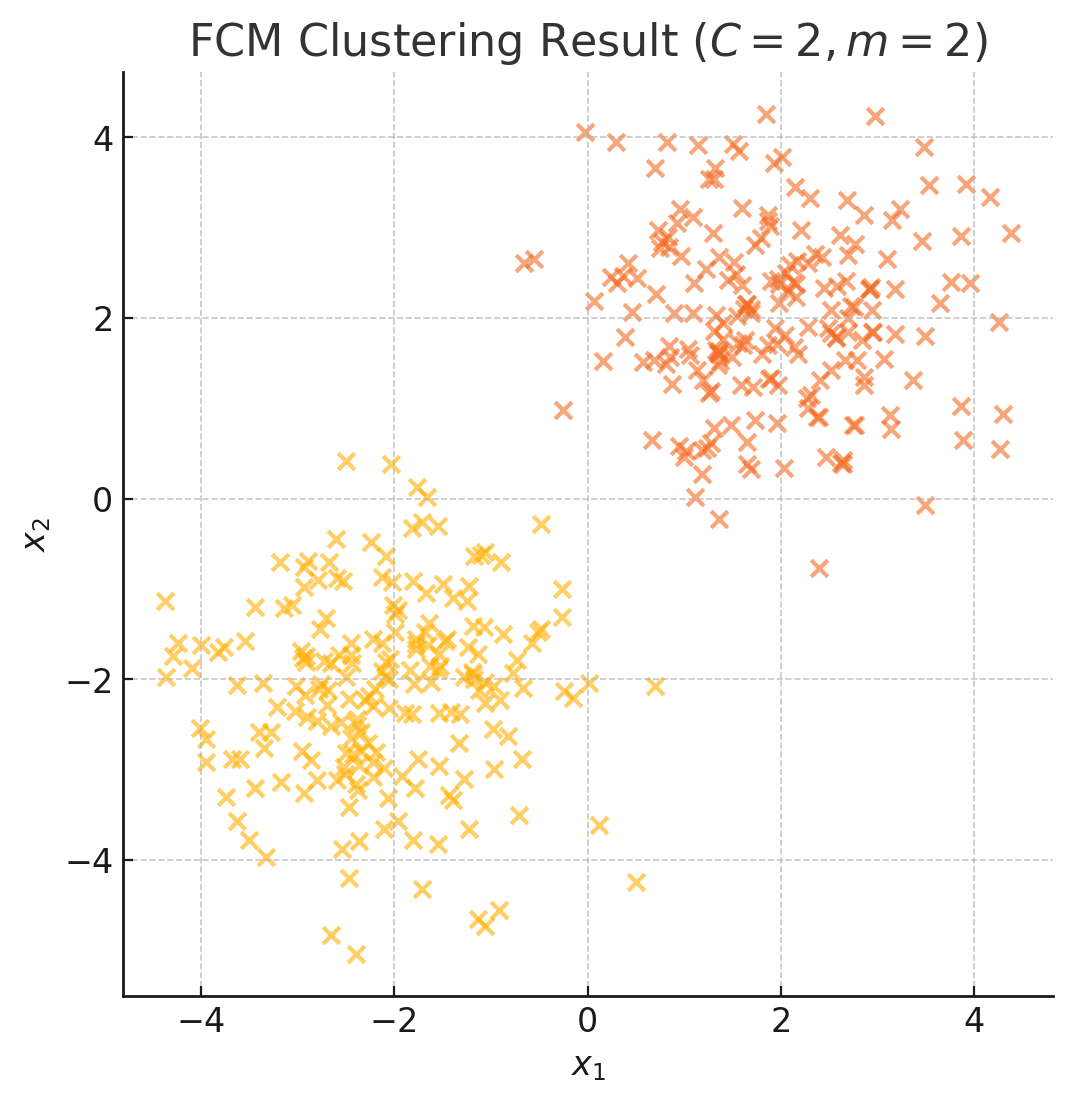
\includegraphics[width=0.7\linewidth]{images/fuzzy_surface.png}
  \caption{Поверхность управления $u^*(e,\dot e)$ нечётым ПИД‐контроллером. Авторский материал}
  \label{fig:fuzzy-surface}
\end{figure}

\begin{example}[Кластеризация методом Fuzzy C‐Means]
Дано облако точек $\{x_i\}_{i=1}^N\subset\mathbb{R}^2$. В FCM минимизируется функционал
\[
  J = \sum_{i=1}^N \sum_{j=1}^C (\mu_{ij})^m \,\|x_i - c_j\|^2,
\]
где $\mu_{ij}\in[0,1]$ — степень принадлежности точки $x_i$ кластеру $j$, $m>1$ — параметр «размытия», $c_j$ — центр $j$-го кластера.  
Итерационные формулы:
\[
  \mu_{ij}
    = \frac{1}{\sum_{k=1}^C \bigl(\|x_i-c_j\|/\|x_i-c_k\|\bigr)^{2/(m-1)}}, 
  \quad
  c_j
    = \frac{\sum_{i=1}^N (\mu_{ij})^m\,x_i}{\sum_{i=1}^N (\mu_{ij})^m}.
\]
\end{example}

\begin{figure}[ht]
  \centering
  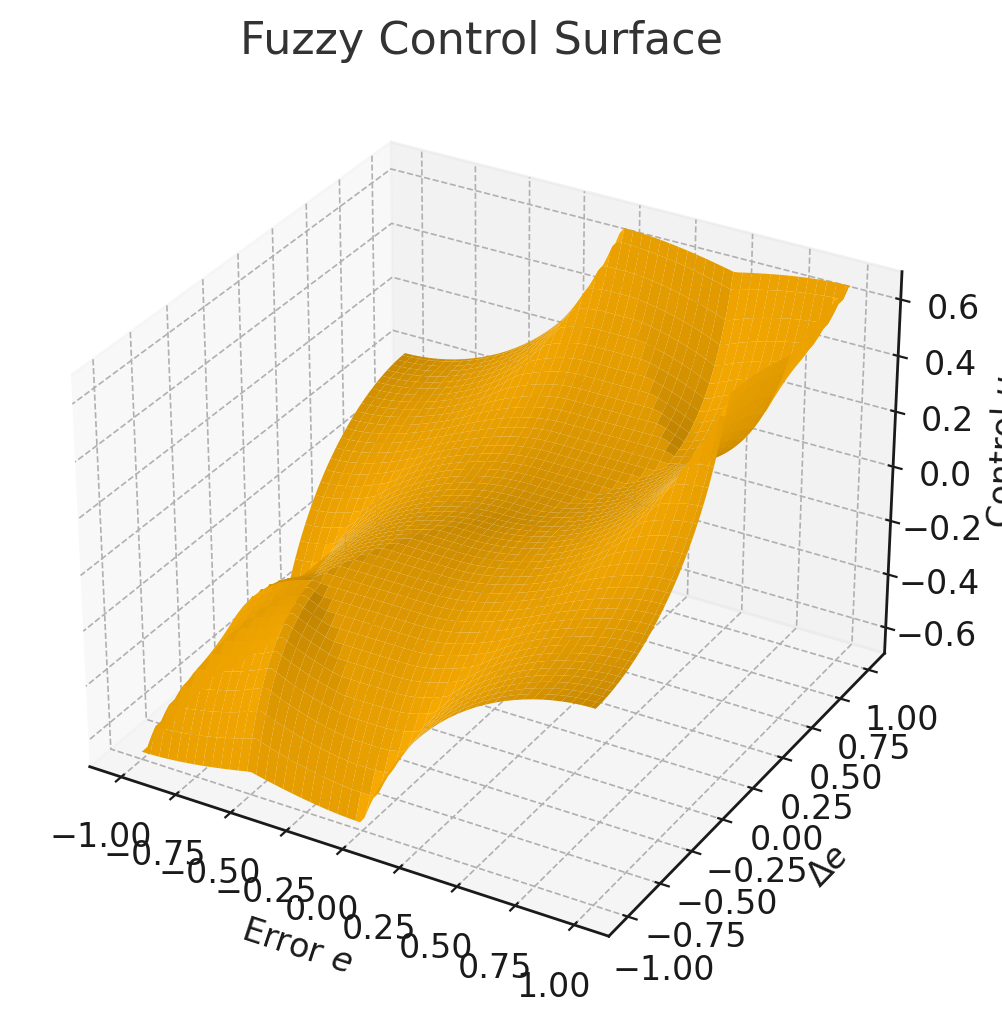
\includegraphics[width=0.7\linewidth]{images/fcm_clusters.png}
  \caption{Результат разбиения точек на $C=2$ кластера методом Fuzzy C‐Means ($m=2$). Авторский материал}
  \label{fig:fcm-clusters}
\end{figure}

\begin{example}[Экспертная система диагностики]
Пусть оцениваются три показателя электродвигателя: температура $T$, вибрация $V$ и шум $S$.  
Каждая переменная имеет термы «низкий», «средний», «высокий» с функциями принадлежности $\mu_{t}(x)\in[0,1]$.  
Пример правила:
\[
  \text{Если }T\text{— высокое}\land V\text{— высокое}\land S\text{— среднее,}
  \text{ то риск отказа — очень высокий}.
\]
Агрегированное нечёткое множество риска $R$ дефаззифицируется в численный уровень $r^*\in[0,1]$.
\end{example}

\subsection{Методы \emph{non--singleton} вывода}

\label{subsec:other_defuzz}

\subsubsection{Метод Мамдани (Mamdani)}
\label{sec:mamdani}

В классическом подходе Мамдани (1975) объединение выводов правил осуществляется путём «обрезки» (операция минимум) или «усечения» исходных выходных функций принадлежности на уровне активации каждого правила. При этом входные данные обычно представлены в виде singleton, и вся неопределённость от измерения «съеживается» в одно число. В результате при одинаковых степенях срабатывания разных правил теряется информация о форме исходного распределения, что может приводить к снижению устойчивости вывода и искажению результирующего нечёткого множества.

В предлагаемом варианте сохраняется непрерывное представление входного сигнала через non–singleton фаззификацию: каждому точечному измерению $x'$ сопоставляется гауссовская функция
\[
  \mu_X(u)
  = \exp\!\Bigl(-\tfrac12\bigl(\tfrac{u - x'}{\sigma}\bigr)^2\Bigr), 
  \quad u\in U,
\]
которая отражает как инструментальную, так и лингвистическую неопределённость. Далее вывод по каждому правилу производится по модифицированной процедуре Мамдани, а дефаззификация — через центр тяжести с учётом обоих распрделений.

\paragraph{Алгоритм с non–singleton фаззификацией}
\begin{enumerate}
  \item \textbf{Фаззификация входа.} Преобразовать каждое наблюдение $x'$ в нечёткое множество с МФ $\mu_X(u)$;
  \item \textbf{Оценка правил.} Для каждого правила $k=1,\dots,m$ вычислить степень активации;
  \[
    w_k \;=\;\sup_{u\in U}\bigl[\mu_X(u)\,\ast\,\mu_{A_k}(u)\bigr],
  \]
  где ‘‘$\ast$’’ — выбранная конъюнкция (например, минимум или произведение).
  \item \textbf{Агрегация выводов.} Построить результирующее нечёткое множество на выходе;
  \[
    \mu_Y(y\mid u)
    = \bigvee_{k=1}^{m}\bigl[w_k \,\ast\, \mu_{B_k}(y)\bigr],
  \]
  где ‘‘$\vee$’’ — дизъюнкция (например, максимум).
  \item \textbf{Дефаззификация.} Рассчитать точечное значение выхода по центру тяжести:
  \[
    y^* 
    = 
    \frac{\displaystyle\iint_{U\times\mathbb R}
      y\,\mu_Y(y\mid u)\,\mu_X(u)\,du\,dy}
         {\displaystyle\iint_{U\times\mathbb R}
      \mu_Y(y\mid u)\,\mu_X(u)\,du\,dy}.
  \]
\end{enumerate}

Такой алгоритм сохраняет информацию о форме входного распределения и повышает устойчивость вывода к шуму и погрешностям измерений, но увеличивает вычислительную сложность до $O(nmP)$, где $n$ — число правил, $m$ — число выходных лингвистических термов, а $P$ — число точек дискретизации множества $U$.

\begin{figure}[H]
  \centering
  \begin{tikzpicture}
    \begin{axis}[
      width=0.8\linewidth,
      xlabel={$u$}, ylabel={$\mu$},
      title={Пересечение двух гауссовских функций принадлежности},
      domain=-4:4, samples=200,
      ymin=0, ymax=1.05,
      ytick={0,1}, yticklabels={0,1},
    ]
      \addplot[thick, draw=red]  {exp(-0.5*((x+1)/1)^2)};
      \addplot[thick, draw=blue] {exp(-0.5*((x-2)/0.5)^2)};
      \addplot[thick, draw=green!80!black, fill=green!20]
        plot [domain=-4:4] {min(
          exp(-0.5*((x+1)/1)^2),
          exp(-0.5*((x-2)/0.5)^2)
        )} \closedcycle;
      \legend{$\mu_1(u)$,$\mu_2(u)$,$\mu_{\cap}(u)$}
    \end{axis}
  \end{tikzpicture}
  \caption{Иллюстрация «усечения» по Мамдани при $\alpha=0.6$. Авторский материал}
\end{figure}


\subsubsection{Метод Такеги–Сугено (Takagi–Sugeno)}
\label{subsubsec:sugeno}

В методе Сугено (1985) результат каждого правила задаётся не нечётким множеством, а аналитической функцией от входных переменных. Это позволяет получить численное выражение для $y^*$ без тройной интеграции дефаззификации.

\paragraph{Основные этапы}
\begin{enumerate}[label=\alph*)]
  \item \emph{Фаззификация.} Каждое входное значение $u_i$ преобразуется в степень принадлежности $\mu_{A_k}(u_i)$;
  \item \emph{Активация правила.} Для правила $k$ вычислить вес.
    \[
      w_k \;=\; T\bigl(\mu_{A_k^1}(u_1),\dots,\mu_{A_k^n}(u_n)\bigr),
    \]
    где $T$ — выбранная T-норма (например, минимум или произведение);
  \item \emph{Численный вывод.} Подставить $u=(u_1,\dots,u_n)$ в линейную функцию
    \[
      f_k(u) = a_{k1}u_1 + \dots + a_{kn}u_n + b_k,
    \]
    получив $y_k = f_k(u)$;
  \item \emph{Агрегация.} Итоговое значение
    \[
      y^* = \frac{\sum_{k=1}^m w_k\,y_k}{\sum_{k=1}^m w_k}.
    \]
\end{enumerate}

\begin{figure}[H]
  \centering
  \begin{tikzpicture}
    \begin{axis}[
      width=0.7\linewidth,
      xlabel={$u$}, ylabel={$y$},
      title={Иллюстрация работы метода Сугено},
      xmin=0, xmax=2, ymin=0, ymax=5,
      xtick={1}, xticklabels={$u_0$},
      ytick={2,4}, yticklabels={$y_2$,$y_1$},
      legend pos=north west,
      legend cell align=left,
      tick align=outside,
    ]
      %--- указываем веса в нижнем правом углу ---
      \node[anchor=south east] at (rel axis cs:0.98,0.02) {$w_1=0.6,\;w_2=0.4$};

      %--- основные графики и легенда ---
      \addplot[thick, red] {3*x + 1};
      \addlegendentry{$f_1(u)$}
      \addplot[thick, blue] {2*x};
      \addlegendentry{$f_2(u)$}
      \addplot[thick, dashed, draw=green!80!black] coordinates {(0,3.2) (2,3.2)};
      \addlegendentry{$y^*$}

      %--- вертикальная линия u = u0 (без легенды) ---
      \addplot[dashed, thick, gray, forget plot] coordinates {(1,0) (1,5)};

      %--- точки пересечения (без легенды) ---
      \addplot[only marks, mark=*, red,   forget plot] coordinates {(1,4)};
      \addplot[only marks, mark=*, blue,  forget plot] coordinates {(1,2)};
      \addplot[only marks, mark=*, green!80!black, fill=white, forget plot]
        coordinates {(0,3.2)};
      \addplot[only marks, mark=*, green!80!black, fill=green!20, forget plot]
        coordinates {(1,3.2)};

      %--- подписи точек ---
      \node[above right] at (axis cs:1,4)   {$(1,4)$};
      \node[below right] at (axis cs:1,2)   {$(1,2)$};
      \node[left]        at (axis cs:0,3.2) {$(0,3.2)$};
    \end{axis}
  \end{tikzpicture}
  \caption{%
    При $u=u_0=1$, весовые коэффициенты $w_1=0.6$, $w_2=0.4$.\\[6pt]
    Это даёт $f_1(1)=4$, $f_2(1)=2$ и 
    $y^*=\dfrac{0.6\cdot4 + 0.4\cdot2}{0.6+0.4}=3.2$. Авторский материал
  }
\end{figure}

\paragraph{Преимущества и ограничения}
\begin{itemize}
  \item Ясная параметрическая форма выхода, удобная для идентификации и оптимизации;
  \item Отсутствие тяжёлой центр-тяжести-дефаззификации на каждом шаге;
  \item Зависимость $f_k(u)$ может плохо соответствовать интуитивно понятным лингвистическим термам.
\end{itemize}


\subsubsection{Метод Цукамото (Tsukamoto)}
\label{subsubsec:tsukamoto}

В методе Цукамото (1979) каждая выходная МФ должна быть монотонной и обратимой. При уровне активации $\alpha_k$ правила вычисляется единственное численное значение $y_k$, после чего все $y_k$ усредняются.

\paragraph{Основные этапы}
\begin{enumerate}
  \item \emph{Фаззификация.} По входным данным $u$ вычислить степень срабатывания $w_k$ каждого правила;
  \item \emph{Инверсия МФ.} Для каждой выходной функции $\mu_{Y_k}(y)$ (монотонной на рассматриваемом диапазоне) найти.
    \[
      y_k = \mu_{Y_k}^{-1}(w_k);
    \]
  \item \emph{Агрегация.} Итоговое значение рассчитывается по формуле:
    \[
      y^* = \frac{\sum_{k=1}^m w_k\,y_k}{\sum_{k=1}^m w_k}.
    \]
\end{enumerate}

\begin{figure}[H]
  \centering
  \begin{tikzpicture}
    \begin{axis}[
      width=0.8\linewidth,
      xlabel={$w_k$}, ylabel={$y_k$},
      title={Обратное преобразование в методе Цукамото},
      xmin=0, xmax=1, ymin=0, ymax=10,
      xtick={0,0.3,0.8,1},
      xticklabels={0,$w_1=0.3$,$w_2=0.8$,1},
      ytick={2,3.8,6.8,8},
      yticklabels={$y_{\min}=2$,$y_1=3.8$,$y_2=6.8$,$y_{\max}=8$},
      legend pos=north west,
      legend cell align=left,
    ]
      % сама линейная функция
      \addplot[thick, purple] {2 + 6*x};
      \addlegendentry{$y_k=\mu^{-1}_{Y_k}(w_k)$}

      % точки для w1 и w2
      \addplot[only marks, mark=*, draw=purple, fill=purple!50] 
        coordinates {(0.3,2+6*0.3) (0.8,2+6*0.8)};

      % подписи рядом с точками
      \node[above right] at (axis cs:0.3,3.8) {$(0.3,\,3.8)$};
      \node[above right] at (axis cs:0.8,6.8) {$(0.8,\,6.8)$};
    \end{axis}
  \end{tikzpicture}
  \caption{%
    Линейная обратная функция $y_k=2+6\,w_k$, \\
    отмечены точки $(w_1,y_1)=(0.3,3.8)$ и $(w_2,y_2)=(0.8,6.8)$. Авторский материал} 
\end{figure}

\paragraph{Преимущества и ограничения}
\begin{itemize}
  \item Итоговое значение $y^*$ определяется без интеграции, сохраняя интерпретируемость выходных МФ;
  \item Необходима строгая монотонность и обратимость каждой функции $\mu_{Y_k}(y)$, что ограничивает гибкость.
\end{itemize}


\subsection{Классификация систем вывода и их свойства}
\label{subsec:classification}
\begin{enumerate}
  \item[] Полный процесс нечеткого вывода состоит из четырёх этапов:
  \item \emph{Фазификация}: $u\mapsto\mu_{A_i}(u)$;
  \item \emph{Агрегация условий}: $t$-норма/ко-норма,
        например, произведение
        \begin{equation}
          w_k=\prod_{i=1}^{n}\mu_{A_{ik}}(x_i);
          \label{eq:tprod}
        \end{equation}
  \item \emph{Композиция правил}: максимум или сумма
        результирующих множеств;
  \item \emph{Дефаззификация}: превращение
        нечёткого вывода в скаляр.  
        Для правила Мамдани чаще всего —
        центроид
        \begin{equation}
          y^\star=\frac{\displaystyle
                     \int_{\mathbb R} y\,\mu_Y(y)\,dy}
                     {\displaystyle\int_{\mathbb R}\mu_Y(y)\,dy}.
          \label{eq:centroid}
        \end{equation}
\end{enumerate}

\subsection{Сравнение метод обучения нейросетей и нечётких систем}
\label{subsec:training_methods}

\paragraph{Нейронные сети}
\begin{itemize}
  \item \textbf{Градиентный спуск} (SGD, Adam, RMSprop) — быстрый локальный поиск;
  \item \textbf{Regularization} (Dropout, BatchNorm, weight decay) для борьбы с переобучением;
  \item \textbf{Transfer learning} — дообучение предобученных моделей;
  \item \textbf{Meta-learning / AutoML} (HyperOpt, Optuna) для поиска архитектуры и гиперпараметров.
\end{itemize}

\paragraph{Нечёткие системы}
\begin{itemize}
  \item \textbf{Экспертное задание MF и правил} — ручная настройка на основе знаний;
  \item \textbf{Алгоритмы типа Wang–Mendel} \cite{Wang1992} для автоматической генерации правил;
  \item \textbf{Эволюционные алгоритмы} (GA, PSO, Differential Evolution) для оптимизации MF и весов правил;
  \item \textbf{Градиентное обучение MF} в ANFIS — backprop через параметры функций принадлежности;
  \item \textbf{Bayesian/BO–тюнинг} (Optuna) — поиск границ MF и структуры базы правил.
\end{itemize}

\begin{table}[H]
\centering\small
\caption{Сравнительный анализ методов обучения}
\begin{tabular}{@{}p{0.25\linewidth}p{0.33\linewidth}p{0.33\linewidth}@{}}
\toprule
\textbf{Метод} & \textbf{Нейросети} & \textbf{Нечёткие системы} \\ \midrule
Градиентный & 
Backprop, Adam, быстрый on-line & 
ANFIS: backprop через MF, редко применяется  \\[2pt]
Эволюционный & 
редко (NeuroEvolution) &
GA/PSO для MF + правил, глобальный поиск \\[2pt]
Bayesian/BO & 
Optuna, Ax, Hyperopt для гиперпарам. &
Optuna для MF, границ правил; медленнее \\[2pt]
Экспертный ввод & 
нет (данные → модель) &
основа для MF, структур правил \\[2pt]
AutoML & 
AutoKeras, AutoGluon &
ограниченно: FuzzyAutoML проекты \\ 
\bottomrule
\end{tabular}
\end{table}

\begin{table}[H]
\centering\small
\caption{Сравнение по методам обучения и свойствам}
\label{tab:nn_fuzzy_training}
\begin{tabular}{@{}p{0.20\linewidth}p{0.36\linewidth}p{0.36\linewidth}@{}}
\toprule
\textbf{Аспект} & \textbf{Нейросети} & \textbf{Нечёткая логика} \\ \midrule
Инициализация & случайные веса, pretrain & заранее заданные MF, пороговые значения \\[4pt]
Обновление & градиентный шаг & GA-прогрессия / Optuna Trial \\[4pt]
Сходимость & зависит от lr, batch size, architecture & зависит от структуры правил, параметров MF \\[4pt]
Глобальный поиск & сложен, требует NeuroEvolution & GA/PSO встроены, естественно \\[4pt]
Автоматизация & AutoML фреймворки & Optuna, но меньше готовых решений \\[4pt]
Интерпретируемость  & пост-хок (LIME, SHAP) & прямая: правила–последствия \\[4pt]
Оценка качества & валидация на hold-out & экспертная и статистическая валидация \\ 
\bottomrule
\end{tabular}
\end{table}

\paragraph{Заключение}
\begin{itemize}
  \item \emph{Нейросети} полагаются на мощные процедуры градиентного обучения и AutoML, но требуют больших данных и пост-хок интерпретации.
  \item \emph{Нечёткие системы} используют комбинацию экспертных знаний и глобального поиска (GA, BO), обеспечивая читаемость, но уступая в зрелости AutoML-сред.
  \item Гибридные подходы (ANFIS, SugenoGPU) берут лучшее из обоих миров: интерпретируемые правила и дифференцируемые MF, обучаемые градиентом, часто в сочетании с Optuna для мета-оптимизации.
\end{itemize}

\subsection{Инструментальные средства и технологии разработки}
\label{subsec:tools}

\subsubsection{Актуальность выбора инструментов}
\label{subsubsec:why_tools}

При разработке нейронечёткой системы с non–singleton входами возникают
ряд взаимосвязанных требований к среде разработки и используемым библиотекам:
необходимость эффективной обработки больших объёмов данных,
высокая вычислительная производительность при сложных интегральных операциях,
а также гибкость в экспериментировании и воспроизводимость результатов.
Одновременно важна прозрачность и удобство отладки, а также лёгкость
интеграции компонентов в единую платформу.

\medskip

\noindent Основные аргументы в пользу продуманного выбора стека:
\begin{itemize}
  \item \textbf{Производительность.} Фазификация non–singleton входов
        требует многократных операций над массивами данных и
        интегральных вычислений с высокой степенью параллелизма.
        Без GPU-ускорения и оптимизированных библиотек
        время вычисления становится неприемлемым;
  \item \textbf{Гибкость.} Экспериментальная платформа должна
        позволять динамически менять архитектуру нейронечёткой модели,
        добавлять новые функции принадлежности, заменять оптимизаторы
        и изменять логику дефаззификации без переписывания кода «с нуля»;
  \item \textbf{Воспроизводимость.} Поддержка управления зависимостями
        (виртуальные окружения, Docker), фиксированные версии библиотек
        и единый конфигурационный формат гарантируют
        идентичность получаемых результатов на разных машинах;
  \item \textbf{Экосистема.} Доступ к большим сообществам разработчиков,
        обширная документация и постоянная поддержка обновлений
        являются залогом долгосрочной устойчивости проекта.
\end{itemize}

\subsubsection{Менеджмент окружения и зависимостей}

Для контроля версий пакетов и изоляции окружения рекомендуются:
\begin{itemize}
  \item \textbf{Conda / mamba.} Гибкое создание виртуальных сред,
        возможность установки как Python-библиотек, так и
        низкоуровневых CUDA-драйверов в одном канале;
  \item \textbf{Poetry.} Современный инструмент для управления
        зависимостями и публикации пакетов, поддерживает lock-файл
        и разрешает конфликтующие версии;
  \item \textbf{Docker.} Контейнер с базовым образом \verb|nvidia/cuda|,
        позволяющий запускать приложение на любом GPU-сервере
        без дополнительной настройки.
\end{itemize}

\subsubsection{Ключевые библиотеки и примеры использования}

\paragraph{Работа с данными}

\emph{pandas} остаётся де-факто стандартом для анализа табличных данных:
интуитивный API, богатый набор функций агрегации, ресэмплирования
и временных индексов.  
Для больших наборов данных применимы \emph{polars} (Rust-ядро,
комбинация ленивых вычислений и multithreading) и \emph{Dask}
(распределённая обработка на кластере).
\begin{center}
  \captionof{listing}{Пример ресэмплирования временных рядов в pandas}
  \label{lst:pandas_resample}
  \medskip
  \begin{minted}[]{python}
import pandas as pd
df = pd.read_parquet("sensor_data.parquet")
df.index = pd.to_datetime(df["timestamp"])
df_resampled = df.resample("100ms").mean().interpolate()
  \end{minted}
\end{center}

\newpage
\paragraph{Численные расчёты: NumPy, SciPy, CuPy, Numba.}

\emph{NumPy} обеспечивает базовые операции над многомерными массивами.
\emph{SciPy} дополняет оптимизацией, интегрированными методами и
статистическими инструментами.  
\emph{CuPy} даёт «drop-in» замену NumPy на GPU,
а \emph{Numba} компилирует критичные фрагменты кода в машинный язык
с поддержкой CUDA-ядр.


\begin{center}
  \captionof{listing}{Пример ресэмплирования временных рядов в pandas}
  \medskip
  \begin{minted}[]{python}
from numba import njit
import numpy as np

@njit
def trap_mf(x, a, b, c, d):
    if x < a or x > d:
        return 0.0
    elif x < b:
        return (x-a)/(b-a)
    elif x <= c:
        return 1.0
    else:
        return (d-x)/(d-c)
  \end{minted}
\end{center}

\paragraph{Машинное обучение и оптимизация}

\emph{PyTorch} служит ядром для тензорной алгебры, CUDA-ускорения,
автоградиента и гибкого построения вычислительных графов.
\emph{scikit-learn} предоставляет baseline-модели, трансформеры данных
и метрики качества.  
\emph{imbalanced-learn} наращивает функциональность scikit-learn 
версиями SMOTE, ADASYN и другими.  
\emph{Optuna} — современный фреймворк для гипероптимизации
с поддержкой прунинга и распределённого хранения экспериментов.


\begin{center}
  \captionof{listing}{Пример Pipeline с SMOTE и RandomForest}
  \medskip
  \begin{minted}[]{python}
from sklearn.pipeline import Pipeline
from sklearn.preprocessing import StandardScaler
from sklearn.ensemble import RandomForestClassifier
from imblearn.over_sampling import SMOTE

pipe = Pipeline([
    ("scale",  StandardScaler()),
    ("smote",  SMOTE(k_neighbors=4)),
    ("clf",    RandomForestClassifier(n_estimators=200))
])
pipe.fit(X_train, y_train)
  \end{minted}
\end{center}

\begin{center}
  \captionof{listing}{Optuna-оптимизация параметров модели}
  \medskip
  \begin{minted}[]{python}
import optuna
def objective(trial):
    n_trees = trial.suggest_int("n_trees", 50, 300)
    max_depth = trial.suggest_int("max_depth", 5, 20)
    clf = RandomForestClassifier(n_estimators=n_trees, max_depth=max_depth)
    score = cross_val_score(clf, X_train, y_train, cv=3).mean()
    return 1 - score

study = optuna.create_study(direction="minimize")
study.optimize(objective, n_trials=50)
  \end{minted}
\end{center}

\subsubsection{Выводы}
\label{subsubsec:tool_summary}
\begin{itemize}
  \item[] В результате подробного обзора выбраны инструменты,
обеспечивающие:
  \item надёжную и воспроизводимую среду (Conda, Docker, GitHub Actions);
  \item высокую производительность при фазификации и дефаззификации
        (PyTorch, CuPy, Numba);
  \item богатый набор средств для работы с данными и их балансировки
        (pandas, polars, imblearn);
  \item гибкие механизмы гипероптимизации и экспериментального
        прототипирования (Optuna, Streamlit).
\end{itemize}

Такой инструментальный стек гарантирует модульность, масштабируемость
и удобство сопровождения проекта нейронечёткой системы
с non–singleton входами
